\begin{frame}
  \frametitle{\#goals}
  \centerline{My goal is that you will get}
  \centerline{The Translog Aha Experience}
\end{frame}

\begin{frame}
  \frametitle{What is a transparency log}
  \centerline{Imagine a list}
  \centerline{
\includegraphics{img/list3_s}}
  \pause
  \centerline{If the list is ever changed, and not merely appended to,
    that will be visible}
\end{frame}

\begin{frame}
  \frametitle{What is a transparency log}
  \centerline{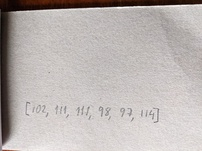
\includegraphics{img/list6_s}}
  \centerline{Adding is fine}
\end{frame}

\begin{frame}
  \frametitle{What is a transparency log}
  \centerline{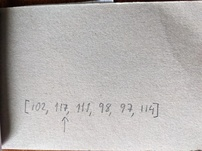
\includegraphics{img/list6mutarrow_s}}
  \centerline{Ooops}
\end{frame}

\begin{frame}
  \frametitle{What is a transparency log}
  \centerline{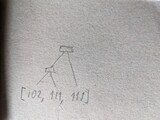
\includegraphics{img/tree3_s}}
  \centerline{Back up and add checksums}
\end{frame}

\begin{frame}
  \frametitle{What is a transparency log}
  \centerline{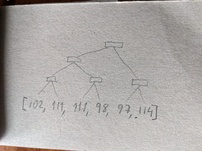
\includegraphics{img/tree6_s}}
  \centerline{In a tree}
  \pause
  \centerline{See https://rgdd.se/tlog0 if this fascinates you}
\end{frame}

\begin{frame}
  \frametitle{What can a transparency log be used for}

  \begin{itemize}
  \item Official documents
  \item Syslog audit trail
  \item Quarantined vulnerability disclosure mailing list
  \item Cryptographic key-usage
  \item Public-key infrastructure and naming systems
  \item Anonymity network relay lists
  \item Source code
  \item Executable binaries
  \item BGP announcements
  \item Ansible playbooks
  \end{itemize}

\end{frame}

\begin{frame}
  \frametitle{What can a transparency log be used for}

  Official documents
  \pause

  Do you have official documents that really shouldn't be tampered
  with, like tax declarations, documents of ownership, evidence in
  law-cases, and news feeds? A transparency log would ensure that any
  removal or modification would be detected.

\end{frame}

\begin{frame}
  \frametitle{What can a transparency log be used for}

  Syslog audit trail
  \pause

  To detect systems that were compromised or mis-used, selected system
  operations could be transparency logged. For example, who accessed
  which medical records and at what time?
\end{frame}

\begin{frame}
  \frametitle{What can a transparency log be used for}

  Quarantined vulnerability disclosure mailing list
  \pause

  Vulnerability dislosure mailing lists sometimes have policies like
  making reported issued public after X days. Transparency logging the
  hash of all incoming reports would ensure that it is not possible to
  skip the disclosure phase without detection. The parties on the
  mailing list would also know if they are not receiving all reports.
\end{frame}

\begin{frame}
  \frametitle{What can a transparency log be used for}

  Cryptographic key-usage
  \pause

  How to detect if a secret signing key gets compromised or mis-used?
  This applies to both the entity owning the key as well as the
  broader public that relies on it. Requiring that signatures are
  transparency logged helps detecting new signature operations.
\end{frame}

\begin{frame}
  \frametitle{What can a transparency log be used for}

  Public-key infrastructure and naming systems
  \pause

  The web's public-key infrastructure consists of trusted third-party
  certificate authorities that vouch for domain names to public-key
  bindings. By transparency logging the issued certificates, it is
  posisble to detect CAs that make mistakes (intentional or not).
  This is usually referred to as Certificate Transparency.

  \begin{itemize}
  \item \url{https://certificate.transparency.dev}
  \item \url{https://www.rfc-editor.org/rfc/rfc6962}
  \end{itemize}

  \pause

  The same idea could be applied to the SSH PKI, and even to create
  alternative naming systems similar to Namecoin or ENS (but with a
  central party that is held accountable).
\end{frame}

\begin{frame}
  \frametitle{What can a transparency log be used for}

  Anonymity network relay lists
  \pause

  Anonymity networks are usually composed of relays that forward
  encrypted traffic. A client that is tricked into using a different
  unique relay list would be trivial to identify. Transparency
  logging the list of relays would detect this type of attack.

  For example, Tor's consensus and the wireguard relay identities of a
  VPN service could be logged.
\end{frame}

\begin{frame}
  \frametitle{What can a transparency log be used for}

  Bootloader
  \pause

  To protect the integrity of a system's boot chain, one can use open
  source firmware (like coreboot) and only permit the operating system
  to start executing if it is transparency logged. This makes it much
  easier to detect backdoors, assess whether up-to-date software is
  running on the bare metal, and so forth.

  \begin{itemize}
  \item \url{https://www.system-transparency.org}
  \end{itemize}
\end{frame}

\begin{frame}
  \frametitle{What can a transparency log be used for}

  Remote attestation
  \pause

  A system that measures different parts of the boot chain into a
  trusted Platform Module (TPM) may allow remote attestations about
  how the system reached its current state. A third-party client
  could enforce that the measured state is transprency logged to
  ensure that the encountered system state is publicly known and
  auditable.
\end{frame}

\begin{frame}
  \frametitle{What can a transparency log be used for}

  Source code
  \pause

  How do you know if you download and build the same source code as
  everyone else?  Or, if the resulting artifact builds reproducibly
  bit-for-bit, which bits are expected?  A transparency log can be
  used to verify that everyone observe the same source code.

  \begin{itemize}
  \item \url{https://go.dev/blog/module-mirror-launch}
  \item \url{https://arxiv.org/pdf/2104.06020.pdf}, page 6 second
    column
  \end{itemize}

\end{frame}

\begin{frame}
  \frametitle{What can a transparency log be used for}

  Executable binaries
  \pause

  How do you know if you download and execute the same binaries as
  everyone else?  A transparency log can be used to verify that
  everyone observe the same binaries. Package managers and software
  updaters would benefit from Binary Transparency.

  \begin{itemize}
  \item \url{https://wiki.mozilla.org/Security/Binary_Transparency}
  \item \url{https://binary.transparency.dev}
  \end{itemize}
\end{frame}


\begin{frame}
  \frametitle{What can a transparency log be used for}

  BGP announcements
  \pause

  BGP is used to find routes from A to B on the internet. Sometimes
  BGP announcements are hijacked to make the traffic take a detour
  into an attacker's networks. A transparency log would ensure that
  suchs highjacks are reliably detected.
\end{frame}


\begin{frame}
  \frametitle{What can a transparency log be used for}

  Ansible playbooks
  \pause

  Ansible is used for configuring systems with so called playbooks. A
  playbook contains information like which programs to install,
  configure and run. By using transparency logged playbooks, the risk
  of executing a malicious playbook without detection decreases.
\end{frame}

%%%%%%%%%%%%%%%%%%%%
\begin{frame}
  \frametitle{Here's what you can do with Sigsum right now}

  \begin{itemize}
  \item<1-> You can sign and verify checksums with a debug tool (if
    you’re willing to get your hands dirty)
  \item<2-> You can interact with a prototype log using curl
  \item<3-> You can detect signature operations with a prototype
    monitor
  \item<4-> You can verify that a log is not misbehaving uising a
    prototype witness
  \end{itemize}
\end{frame}

\begin{frame}
  \frametitle{What would you do with a transparency log?}

  What use do you see for such a thing?
  \pause

  Find Sigsum people in \#sigsum @ OFTC.net and matrix.org and on the
  sigsum-general@lists.sigsum.org mailing list
\end{frame}
